\documentclass[11pt]{article}
\usepackage[utf8]{inputenc}
\usepackage[T1]{fontenc}
\usepackage{amsmath}
\usepackage{amsfonts}
\usepackage{amssymb}
\usepackage[version=4]{mhchem}
\usepackage{stmaryrd}
\usepackage{graphicx}
\usepackage[export]{adjustbox}
\graphicspath{ {./images/} }
\usepackage{hyperref}
\hypersetup{colorlinks=true, linkcolor=blue, filecolor=magenta, urlcolor=cyan,}
\urlstyle{same}

\begin{document}
Venture Capital

Venture capital is the most well-known category of private equity. Venture capital focuses on equity or equity-like claims of enterprises that are early stage in terms of growth. They are attempting to grow into large firms but have not yet established substantial and reliable revenues.

The foundation of VC is the underlying start-up businesses and the entrepreneurs who create and build them. Venture capitalists provide financing for these businesses using their own capital and the capital of their investors. Venture capitalists are not passive investors. Once they invest in a company, they take an active role either in an advisory capacity or as a director on the board of the company. They monitor the progress of the company, implement incentive plans for the entrepreneurs and management, and establish financial goals for the company. Besides providing management insight, venture capitalists usually have the right to hire and fire key managers, including the original entrepreneur. They also provide access to consultants, accountants, lawyers, investment bankers, and, most important, other businesses that might purchase the start-up company's product.

Venture capitalists are involved in numerous stages of a firm's growth. Different financing needs are required for each of these stages, and different product technology is found at each stage. In terms of company characteristics, start-up companies generally have a new or innovative technology that can be exploited with the right amount of capital. The management of the company is typically idea-driven rather than operations-driven. A proven revenue model may not yet be established, and the capital consumption is probably high.

The cash flows from VC are related to the operations of these nascent firms and are typically expected to be negative for several years. The cash burn rate of a business describes the speed with which cash is being depleted through time and can be used to project when the organization will deplete its cash and require outside funding. The time until the cash runs out is estimated by dividing the current cash balance by the organization's cash burn rate. For example, a company that has $\$ 30$ million of cash and a burn rate of $\$ 2$ million per month either needs new cash injections in 15 months or needs to reduce its burn rate.

Banks, other lending institutions, and the public stock market are generally unwilling to provide capital to support business plans of firms without collateral or without reasonably high probabilities of positive cash flows in the short run. As the source of equity financing to start-up companies, VC is risky, illiquid, and backed by unproven ideas. The VC investment strategy is to strive for very high rates of return to compensate for the considerable risks.

\section*{Securities and Goals Used in Venture Capital}
Venture capital securities are the privately held stock, preferred stock, or equity-linked securities that venture capitalists obtain when investing in business ventures that are striving to become larger and to go public. Investors in venture capital securities must be prepared to invest for the long haul; investment horizons may be as extended as 5 to 10 years. During this time, venture capitalists often take active roles in providing managerial guidance and, to varying degrees, exercising managerial control. The ultimate goal of the venture capitalist is for the venture to be successful, usually to the point that the firm can exit the investment at a profit. VC exits typically focus on going public (i.e., conducting an initial public offering of the company's securities), but can also include sales to acquiring firms or even a leveraged recapitalization, where the proceeds from the debt are paid to the venture capitalist. Successful start-up companies funded by venture capital include Cisco Systems, Google, Microsoft, and Genentech.

Attractive VC investment opportunities can be difficult to assess and are usually concentrated in a few high-technology sectors, often resulting in a relatively high number of small investments. Returns stem from taking large risks to develop new businesses and concentrating efforts and capital through several incremental funding rounds. The goal is to build companies that can be sold or taken public with a high multiple of invested capital. These few big wins need to compensate for many failures. VC-funded companies can be seen as works in progress, with intermediate stages of completion. These stages of completion are often distinguished by milestones, such as rounds of financing (rounds A, B, and C) or, in the case of biotech companies, phases of clinical trials (phases I, II, and III). In this respect, they are development projects that cannot be prematurely exited without risking the loss of most, if not all, of one's invested capital. Thus, VC transactions should be viewed as long-term investments.

Venture capitalists usually invest in the convertible preferred stock of the start-up company. Investment structures used by venture capitalists include convertible preferred equity, convertible notes, or debentures that provide for the conversion of the principal amount of the note or bond into either common or preferred shares at the option of the venture capitalist, or other positions such as warrants.

Convertible preferred stock is used by VC investors to provide higher priority than common stock along with an implicit call option to share in upside potential similar to the upside potential of equity. In other words, venture capitalists have the option to convert their shares to common stock when exiting via an initial public offering (IPO) and are the favored manner of investment because they are senior to common stock in terms of dividends, voting rights, and liquidation preferences. Convertible notes and debentures may also allow conversion upon the occurrence of an event, such as a merger, an acquisition, or an IPO. There may be several rounds (or series) of preferred stock financing before a successful start-up company goes public.

Venture capitalists sometimes receive warrants to purchase the common equity of the start-up company, as well as stock rights in the event of an IPO.

VC funding by venture capitalists does not typically involve straight debt (i.e., nonconvertible). Venture capitalists gain control of a company over time through a series of equity investments. Venture capitalists typically provide not only financing for building businesses but also industry know-how, relevant contacts, and management expertise. Returns stem from building companies and from managing growth. The investments can be relatively small and are overwhelmingly equity or quasi-equity financed, with little or no leverage. Successful exit strategies usually require VC managers to secure follow-on financing.

\section*{The Option-Like Payout of Venture Capital}
The venture capitalist has a simple binary choice with respect to every potential investment in a start-up business: Invest or don't invest. Investing in a start-up company is similar to the purchase of a call option. The price of the option is the capital that the venture capitalist invests in the start-up company. If the company fails, the venture capitalist forfeits the option premium-the capital invested. However, if the start-up company is successful, the venture capitalist shares in all of the upside, much like a call option.

Most start-ups fail. Clearly, this investment class is not for the fainthearted. Given that venture capitalists are dealing with nascent companies that may or may not burst onto the scene (some just burst), a wide range of returns should be expected. When a company does well, it can result in dramatic upside gains, like a 20-\\
bagger, for its VC investors. The term 20-bagger indicates a company that appreciates in value 20 -fold compared to the cost of the VC investment. This return pattern is similar to a call option and tends to post a return pattern with a large positive skew and a large positive value of kurtosis.

\section*{History of Venture Capital}
Institutional investing in VC remained limited until 1979, due in part to the so-called prudent person standard, or prudent man rule, in the United States. The prudent person standard is a requirement that specifies that the levels of care that should be exercised in particular decision-making roles, such as investment decisions made by a fiduciary, be equal to or greater than the care that a prudent person would exercise for his or her own portfolio. Prudent person rules were established to ensure competent investment decision-making with regard to the large and growing pension assets of U.S. corporations.

The prudent person standard or rule as interpreted prior to 1979 effectively prohibited U.S. pension funds from investing in venture capital funds because of their illiquidity and risk. In 1979, a clarification of the prudent person rule in the United States indicated that venture capital and other high-risk investments should not be considered on a stand-alone basis but on a portfolio basis. Thus, an investment with considerable total risk may be prudent if the marginal contribution of that investment to the risk of the portfolio is reduced through diversification. In addition, the rule clarified that the prudent person test should be based on an investment review process, not on the ultimate outcome of investment results. Therefore, as long as a pension fund investment fiduciary follows sufficient due diligence in considering the portfolio effects of investing in venture capital, the prudent person test is met. The change in the prudent person standard was to base analysis on a portfolio basis (rather than a standalone basis) and to test for prudence based on analysis (rather than outcome), allowing U.S. pension funds for the first time to wholly endorse and engage in venture capital investing. In doing so, it opened venture capital to a vast source of capital: retirement assets.

\section*{Angel and Other Very Early Stages of Venture Capital}
Although some VC firms classify themselves by geography or industry, by far the most distinguishing characteristic of VC investing is the stage of financing. However, the names and descriptions of these stages are not universal. Further, some investors do not differentiate between VC and growth equity, especially in the description of stages. This section does not include those stages that are viewed as growth equity.

Angel investing refers to the earliest stage of venture capital, in which investors fund the first cash needs of an entrepreneurial idea. Angel investors often come from F \& F-that is, friends and family. But sometimes venture capitalists include a third $F$, for fools. At this earliest stage of the venture, typically a lone entrepreneur has just an idea, possibly sketched out at the kitchen table. There is no formal business plan, no management team, no product, no market analysis, just an idea.

In addition to family and friends, angel investors can be wealthy individuals who dabble in start-up companies. Many angel investors are successful businesspeople themselves who may prefer to focus their investments in the industry in which they have built their careers, so that they can offer industry-specific skills or analysis to the entrepreneur. This level of financing is typically done without a private placement memorandum or subscription agreement. It may be as informal as an agreement written on a cocktail napkin. Yet without the angel investor, many ideas would wither on the vine before reaching more traditional venture capitalists.

At the angel stage of financing, the task of the entrepreneur is to begin the development of a prototype product or service. The entrepreneur drafts or revises a business plan, assesses market potential, and possibly even assembles some key management team members. No marketing is done at this stage. This stage often includes or leads to alpha testing of the product or service. Alpha testing is the process of analyzing a product or service to determine its ability to perform its tasks, potentially under laboratory-like conditions, to generate feedback for developers.

The amount of financing at this stage is typically very small: $\$ 50,000$ to $\$ 500,000$. Any more than that would strain family, friends, and other angels. The money is used primarily to flesh out the concept to the point at which an intelligent business plan can be constructed.

The seed capital stage is typically the first stage where institutional investors commit their capital into a venture and is typically prior to having established the viability of the product. At this stage, a business plan is completed and presented to outside investors. Some members of the management team have been assembled at this point, and the entrepreneur and a small team have performed a market analysis and addressed other parts of the business plan. Financing is provided to complete the product development and possibly begin initial marketing of the prototype to potential customers.

This seed-capital phase of financing usually raises $\$ 1$ million to $\$ 5$ million. At this stage of financing, a prototype is developed and product testing begins. This is often referred to as beta testing, in which a prototype is sent to potential customers free of charge to get their input into the product's viability, design, and userfriendliness.

Very little, if any, revenue has been generated at this stage, and the company is definitely not profitable. Venture capitalists invest in this stage based on their due diligence of the management team, their own market analysis of the demand for the product or service, the viability of getting the product to market while there is still time and no other competitor, the additional management team members who need to be added, and the likely timing for additional rounds of capital from the same investors and/or new investors. Unfortunately, the entrepreneur might have to rely on angel investors through this stage as well.

\section*{First-Stage, Start-Up, and Early-Stage Venture Capital}
The first-stage, start-up stage, or early-stage of venture capital begins when the start-up company has a viable product that has been beta tested and involves testing of the second-generation prototype with potential end users and funding after seed capital but before commercial viability has been established. Typically, a price or fee is being charged for the company's product or service. Revenues are being generated, and the product or service is now demonstrating its commercial viability. These early VC financing stages usually require investment totaling $\$ 2$ million or more.

Start-up, first-stage, and early-stage financing is typically used to build out commercial-scale manufacturing services. The product is no longer being produced out of the entrepreneur's garage or some vacant space above a store. The company is now a going concern with an initial, if not complete, management team. At this stage, at least one venture capitalist is sitting on the board of directors of the company. In addition, the business and marketing plans are refined, manufacturing has begun, and initial sales have been established.

The goal of the start-up venture is to achieve market penetration with its product. Some of this will have been accomplished with the beta testing of the product. However, additional marketing must now be done. In addition, distribution channels should be identified by now, and the product should be established in these channels. Reaching a break-even point is the financial goal.

\section*{Second and Later Stages of Venture Capital}
Second- or late-stage/expansion venture capital begins as the start-up company may have generated its first profitable quarter or be near the point of breaking even, and the company and its products are demonstrating commercial viability. Additional terms for the latter stages of VC (before reaching the classification of equity growth) can include third stage and formative stage. The number and names of further stages depend in part on whether a distinction is being made between venture capital and growth equity. Cash flow management is critical at this stage, as the company is not yet at the level where its operating cash flows alone can sustain its own growth.

At this late-stage/expansion VC stage, the start-up venture incurs the growing pains of all successful companies. The future is bright, but working capital is short. Sales and receivables are growing, but the receivables have not yet been translated into a solid and stable cash flow. The start-up may need additional working capital because it has been focusing on product development and product sales but now finds itself with a huge backload of accounts receivable that it must collect from customers. Inevitably, start-up companies are very good at getting the product out the door but very poor at collecting receivables and turning sales into cold, hard cash. Also at this stage, market penetration has been established, and the company has met some initial sales goals. A break-even point has been achieved, and the company is now starting to generate profits, even though its cash is still lagging.

This is when expansion capital can help. Late-stage venture financing helps the successful start-up get through its initial cash crunch. Eventually, the receivables will be collected, and sufficient internal cash will be generated to make the start-up company a self-sustaining force. Until then, one more round of financing may be needed.

Mezzanine venture capital, or pre-IPO financing, is the last funding stage before a start-up company goes public (via an IPO) or is sold to a strategic buyer (via a buyout). At this point, a second-generation product may already be in production, if not distribution.

The financing at this stage is considered bridge or mezzanine financing to keep the company from running out of cash until the IPO or strategic sale. At this stage, the company is a proven winner with an established track record.

Mezzanine financing is halfway between equity and secured debt. Mezzanine financing may be in the form of convertible debt. In addition, the company may have sufficient revenue and earning power to qualify for a traditional loan. Mezzanine financing may also be used to buy out earlier investors and pay for other costs incurred before going public.

\section*{The J-Curve for Private Equity Projects}
The session Quantitative Foundations discusses the concept of the J-curve in private equity, based on accounting conventions, including prompt recognition of early losses and deferral of unrecognized gains. The initial years of a start-up tend to generate a reported accounting-based loss. Money is spent in development, such as turning an idea into a prototype product and beta testing the product with potential customers. Little or no revenue is generated during this time, causing the initial dip in reported performance. Note, however, that the money being spent in development is being spent with the assumption that it is an investment that is creating value for the firm. In an economic sense, the firm may not be losing money, but rather exchanging cash for assets such as information, even if traditional accounting methods do not recognize the information as an asset on the balance sheet. Management believes that the firm is being made more valuable by the development work. It may only be in an accounting sense that the firm is sure to lose money at this stage.

Additional rounds of financing may be needed to get the company to generate cash and profit. Once critical mass is achieved-when products are sold, when sales are turned into profits, and when accounts receivable are turned into cash-the company turns a profit using traditional accounting. As the company realizes its profit potential, it enters into the higher range of profits on the right-hand side of the J-curve. The ultimate goal is at the rightmost part of the J-curve, when the startup company achieves a public offering and the venture capitalists can exit the deal successfully.

The internal rates of return (IRRs) in the next exhibit, except for the rightmost IRR, are generally computed as interim IRRs. Each interim IRR is therefore based on the nonmarket value (net asset value) that was estimated at that point in time. The Life Cycle of a Start-Up Company and the J-Curve includes labels for the typical stages at various points on the curve. The concept of a J-curve for private equity funds is discussed in the session, Private Equity Funds.

\begin{center}
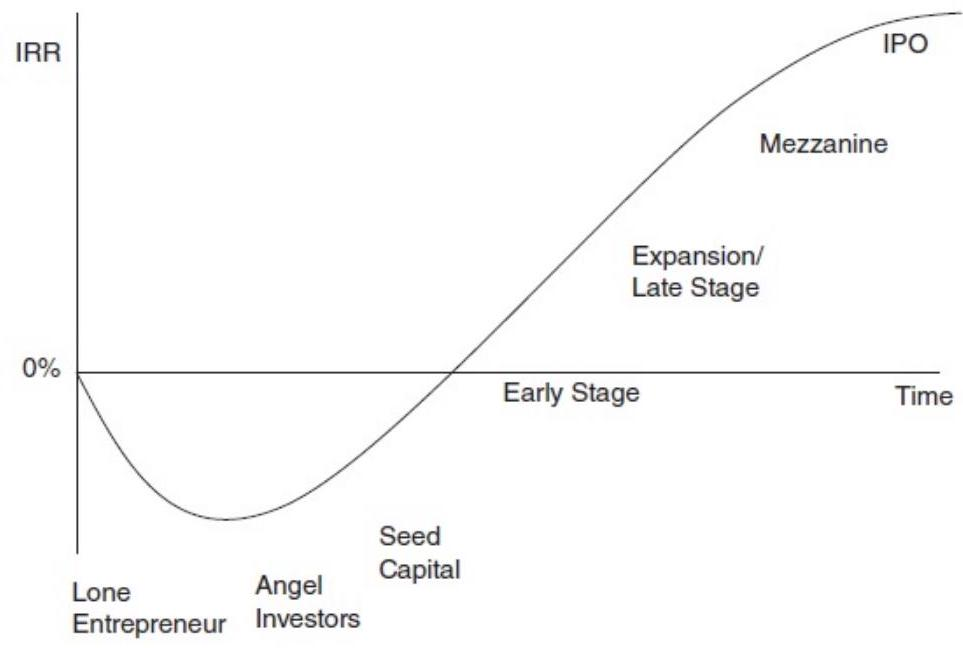
\includegraphics[max width=\textwidth]{2024_04_10_d4c2572c2ae315d9c9f2g-5}
\end{center}

The Life Cycle of a Start-Up Company and the J-Curve

\section*{The Valuation of Venture Capital Companies Based On Operating Income}
Valuation of venture capital is challenging because it depends on the company's operating and financing stage. As listed previously, the stages can be broadly classified into three categories:

\begin{itemize}
  \item Angel stage: Financial projections tend to be inaccurate in this stage, as many companies do not yet earn substantial revenues. The valuation methods used in this stage revolve around identifying key risk factors. The financial valuation of the company increases as the risk elements are resolved.
  \item Growth stage: In this stage, the company has a proven concept and would have generated revenue. Their financial and operating metrics can be used for comparable analysis against similar publicly traded firms. Another popular valuation method is the venture capital method, which uses the potential exit value of a company and the target return of an investor to back into a post-money valuation. This method is described in equation 1 below.
  \item Late stage: In this stage, the company has a proven operating track record, which allows for more accurate financial projections and scenario analysis. A mix of discounted cash flow analysis and analysis of comparable firms may be used to determine the valuation.
\end{itemize}

While, in theory, the value of an investment is the sum of the discounted cash flows, in the case of VC the cash flow projections over long periods of time may be too unreliable to form the basis of a valuation. This section uses a simple multiple of operating income to illustrate the types of rule-of-thumb methods that can be used to estimate the values of highly speculative ventures.

Valuation is also complicated by the lack of appropriate comparisons, which explains why venture capitalists carry out more extensive sector/product due diligence and more limited financial due diligence, compared to other private equity managers such as growth equity or buyout managers. A popular expression of VC worth is enterprise value. Enterprise value is the total value of the company, which adds the equity value of the firm to its outstanding debt and subtracts the cash on the firm's balance sheet. This definition leaves the question of the method of asset valuation unanswered.

The valuation of venture capital-backed firms is challenging, because a wide variety of valuation methods can be used depending on the operating and financing stage of the company. In this section we will focus on valuation based on EBITDA and EBITDA multiples when reliable estimates of long-term cash flows are possible (although other valuation metrics are often used in addition to or in place of EBITDA multiples). For companies with negative EBITDA, revenue multiples are typically used.

EBITDA is a firm's earnings or operating income before interest, taxes, depreciation, and amortization and is therefore used as a measure of before-tax cash flow rather than being a net-of-debt measure. EBITDA multiples are general levels of the perceived ratio between the enterprise value of a firm's assets and its estimated or projected earnings before income taxes, depreciation, and amortization. Thus, the enterprise value can be expanded into the product of the EBITDA and the EBITDA multiple.

One method of modeling the tremendous uncertainty of future value is to discount the projected enterprise value (projected to the estimated point of exit) with a very high required rate of return. VC investors target high IRRs. The reason is simple: there is substantial risk in funding a nascent company with brand-new technology relative to investments in more established companies with regular and predictable cash flows. These required rates of return are typically entitled IRRs consistent with the focus of IRR as a metric for private investments. Equation 1 calculates the value of the venture as a discounted analysis of the enterprise value.


\begin{equation*}
\text { Value of Venture }=(\text { EBITDA } \times \text { EBITDA multiple }) /(1+\mathrm{IRR})^{T} \tag{1}
\end{equation*}


where IRR is the investor's required rate of return and $T$ is the number of years estimated before exit.

Consider a VC investor contemplating a \$4 million investment in a venture targeted to take six years to reach the point of being bought out or going public. The investor requires a 60\% IRR, given the highly uncertain nature of the venture and the risk that the venture will not succeed. The investor projects an EBITDA of $\$ 20$ million (if successful) and an EBITDA multiple of 7.5. Inserting these values into Equation 1 generates:

Value of Venture $=(\$ 20$ million $\times 7.5) /\left(1.60^{6}\right)=\$ 8.94$ million

Taking into consideration the percentage of the firm that the investor will own, the costs of providing oversight and managerial assistance, and any other existing claims to the firm such as indebtedness, the VC investor must decide whether the $\$ 8.94$ million discounted enterprise value warrants the $\$ 4$ million investment.

\section*{Discount Rates Used in Venture Capital}
Venture capitalists typically use a high discount rate when valuing startup firms. These discount rates can range from $30 \%$ to $70 \%$. ${ }^{1}$ Sanjai Bhagat (2014). Why do venture capitalists use such high discount rates? Journal of Risk Finance 15 (no. 1). Discount rates will be higher for younger and more risky companies and lower for more mature and less risky companies. During the early phase, discount rates of $50 \%$ to $70 \%$ are common. ${ }^{2}$ Ibid The discount rate decreases to $30 \%$ to $60 \%$ as the startup progresses from the first through to the fourth stage. ${ }^{3}$ Ibid The intuition is that a company that is further along the company life cycle is likely to be more mature and established, and hence more likely to exit through an IPO or acquisition. Using the database of Crunchbase, ${ }^{4}$ Crunchbase is an online portal that captures information about private companies and funding rounds. For the article, the author's sample consists of over 15,000 US-based technology companies founded between 2003 and 2013. Rowley (2017) compiled the cumulative proportion of exits by stages. The exhibit Cumulative Proportion of Acquired Companies by Stages shows that the cumulative proportion of acquired companies increases at the later stages of equity raising.

Cumulative Proportion of Acquired Companies by Stages

\begin{center}
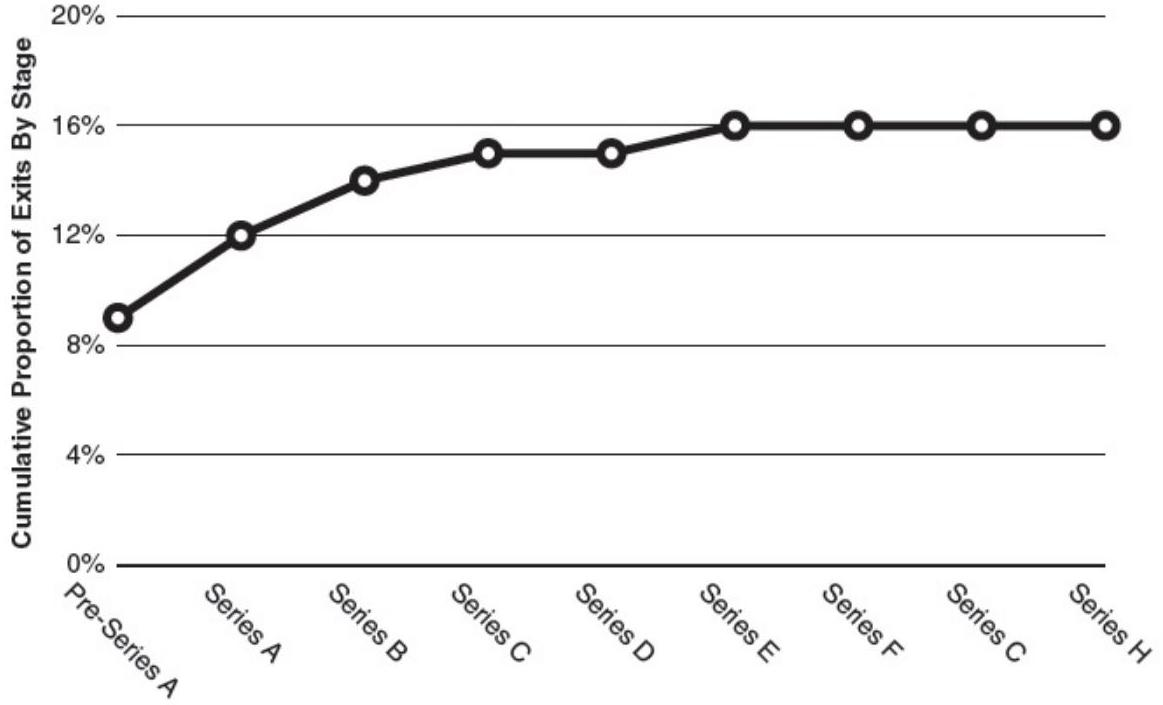
\includegraphics[max width=\textwidth]{2024_04_10_d4c2572c2ae315d9c9f2g-7}
\end{center}

Source: How likely your startup is to get acquired at any stage (2017). Data Source: \href{https://techcrunch.com/2017/05/17/heres-how-likely-your-startup-is-to-getacquired-at-any-stage/}{https://techcrunch.com/2017/05/17/heres-how-likely-your-startup-is-to-getacquired-at-any-stage/}.

Other reasons for high discount rates are:

\begin{itemize}
  \item Illiquidity. Investments made by VC are illiquid until an exit through IPO or acquisition. At the early stages, the lock-up period is longer than in later stages, thus higher expected returns are requested.
  \item Early-stage venture capitalists are typically active investors who make substantial time commitments to their portfolio companies. They may help to build the management team, product design, and provide access to customers or suppliers. Hence, the discount rate may also reflect compensation to the venture capitalists for these efforts.
  \item Adjustment of founder's bias. Founders often provide an upward bias to projections of cash flow for their projects. A higher discount rate may adjust for this bias.
\end{itemize}

\section*{Pre- and Post-Money Valuation}
Pre-money valuation is the enterprise value of a company that is negotiated between the investor and the shareholders of the company prior to a new investment. Pre-money valuation (PRE) is typically used in term sheets and in discussion with the company's founders or investors because the investment amount from the new round of equity raising may fluctuate. It may be challenging to estimate PRE, because it may sometimes not be derived from accounting measures such as revenue, free cash flow, or EBITDA. This is particularly true in the case of early-stage companies with no revenue. In addition, the past valuation of comparable firms can be used as reference points. Ideally, the comparable firms operate in the same sector, same region, and are in a similar stage of their venture capital funding cycle. Furthermore, PRE may be influenced by market conditions such as the amount of capital competing to invest into the company.

Post-money valuation is the enterprise value of the company immediately following a new investment. For example, a venture capital investor (VC investor) makes an investment (NEW MONEY) into a startup. The post-money valuation (POST) of the startup is:


\begin{equation*}
\text { POST }=\text { PRE }+ \text { INVESTMENT } \tag{2}
\end{equation*}


The ownership proportion of the VC investor is:


\begin{equation*}
\text { Ownership = INVESTMENT } / \text { POST } \tag{3}
\end{equation*}


VC investors should keep in mind that their ownership could be diluted in the future due to future equity raising, conversion of convertible debt into equity, and the issuance of stock options to management.

\section*{Venture Capital Business Plans}
How does a venture capitalist select investments? The most important document to a venture capitalist deciding whether to invest in a start-up company is the business plan of the entrepreneur. The venture capital business plan should clearly state the business strategy, identify the niche that the new company will fill, and describe the resources needed to fill that niche, including the expenses, personnel, and assets. It must be comprehensive, coherent, and internally consistent. The business plan of the entrepreneur has two key objectives: (1) to provide the information necessary to attract financing from a venture capitalist, and (2) to serve as an internal game plan for the development of the start-up company.

Business plans should typically have an executive summary and sections that analyze or detail the plans for the market, the product or service, intellectual property rights, the management team, operations, the prior operating history, financial statement projections, the amount of and schedule for financing, and exit opportunities.

The exit plan describes how venture capitalists can liquidate their investment in the start-up company to realize a gain for themselves and their investors. Facilitating exit strategies is a way venture capitalists can add value beyond providing start-up financing. Venture capitalists often have many contacts within established operating companies. An established company may be willing to acquire the start-up company for its technology as part of a strategic expansion of its product line (i.e., an exit based on a buyout). Additionally, venture capitalists maintain close ties with investment bankers. These bankers are necessary if the start-up company decides to seek exit via an IPO. In addition, a venture capitalist may ask other venture capitalists to invest in the start-up company. This helps to spread the risk and also provides additional sources of contacts with operating companies and investment bankers.


\end{document}